\subsection{The Dou et al.\ regime: detectable deviations, still no punishment}
\label{sec:dou}

We next replicate the \citet{dou2025} setting: their calibration
($\sigma_u=0.1$, $\theta=0.1$) with $\alpha=0.05$, as in
\citet{esquinas2026} (their own baseline is $\alpha=0.01$; see
Section~\ref{sec:faithful}), 10 values, a 15-point order grid
per value spanning the cartel-to-Nash range plus 10\%, and the lagged price and
value as state, at $\xi=0$ and at $\xi=500$, where Proposition~\ref{prop:snr}
puts a best-response deviation at about 625 noise standard deviations. Each
trader has its own Q-table, as in the paper's description and the primary
specification of \citet{esquinas2026}. At $\xi=500$ the price state bins the
lagged price over the range the order grid can produce, like the price grid
of \citet{dou2025}; Appendix~\ref{app:binning} shows that a state binned in
units of noise saturates in this regime and reports both versions.
Table~\ref{tab:dou} and Figure~\ref{fig:dou} report the results.

\paragraph{Levels.} Forward-looking learners with price memory reach
$\Delta=\KyleStratDeltaInt$ at $\xi=0$ and $\DouStratDeltaInt$ at $\xi=500$. With
the noise-unit state, the $\xi=500$ value is $0.31$, matching the $0.31$ that
\citet{esquinas2026} report for separate Q-tables in this regime. Our $\xi=0$
value is below their $0.72$; a likely reason, which we have not tested, is the
training horizon: their runs last $5\times10^8$ periods, ours $1.5\times10^7$.

\paragraph{No punishment, even when deviations are glaring.} In both regimes
the forward-looking learners ignore noise shocks: a shock as large as a full
best-response deviation (515 noise standard deviations at $\xi=500$) changes
next-period intensity by $\DouStratShock\pm\DouStratShockCI\%$ of $\beta^N$ at
$\xi=500$, and forced deviations draw no reaction from rivals
($\DouStratRival\pm\DouStratRivalCI\%$) and pay. Detectability is necessary
for punishment but not sufficient: separate-table Q-learners do not discover
trigger strategies within our horizon even when deviations are hundreds of
standard deviations large.

\paragraph{The placebo.} Myopic learners under-trade more than forward-looking
ones at $\xi=0$ ($\KyleMyopicDeltaInt$ versus $\KyleStratDeltaInt$), as in the
standard Kyle experiments, and less at $\xi=500$ ($\DouMyopicDeltaInt$ versus
$\DouStratDeltaInt$). Neither shows a meaningful reaction to shocks or
deviations, so these level differences are not about punishment.

\begin{table}[t]
  \centering
  \small
  \resizebox{\linewidth}{!}{\begin{tabular}{llccccc}
\toprule
$\xi$ & Separate Q-tables & $\Delta$ intensity & $\Delta$ profit & Shock response & Rival reaction & Seeds \\
\midrule
0 & $\gamma=0.95$, remembers price & $0.475 \pm 0.003$ & $0.59 \pm 0.04$ & $0.45 \pm 0.58$ & $-0.66 \pm 0.50$ & 1 \\
0 & $\gamma=0$ (myopic placebo) & $0.632 \pm 0.002$ & $0.74 \pm 0.04$ & $0.27 \pm 0.54$ & $0.32 \pm 0.58$ & 1 \\
0 & $\gamma=0.95$, no memory & $0.37 \pm 0.02$ & $0.50 \pm 0.05$ & $0.00 \pm 0.00$ & $0.00 \pm 0.00$ & 1 \\
500 & $\gamma=0.95$, remembers price & $0.476 \pm 0.002$ & $0.64 \pm 0.01$ & $-0.00 \pm 0.49$ & $-0.48 \pm 0.61$ & 2 \\
500 & $\gamma=0$ (myopic placebo) & $0.130 \pm 0.002$ & $0.21 \pm 0.01$ & $0.59 \pm 0.40$ & $0.47 \pm 0.46$ & 1 \\
500 & $\gamma=0.95$, no memory & $0.24 \pm 0.02$ & $0.36 \pm 0.03$ & $0.00 \pm 0.00$ & $0.00 \pm 0.00$ & 1 \\
\bottomrule
\end{tabular}}
  \caption{\citet{dou2025} calibration with separate Q-tables
  ($1.5\times10^7$ periods, 100 markets per seed). Shock response: change in
  per-trader intensity one period after a noise shock equal to one
  best-response deviation, in \% of $\beta^N$. Rival reaction: change in
  rivals' intensity one period after a forced best-response deviation, in \%
  of $\beta^N$. At $\xi=500$ the price state uses grid-range binning. The
  informativeness index is omitted because at $\xi=500$ the Nash and cartel
  informativeness both equal one to four decimals. 95\% CIs.}
  \label{tab:dou}
\end{table}

\begin{figure}[t]
  \centering
  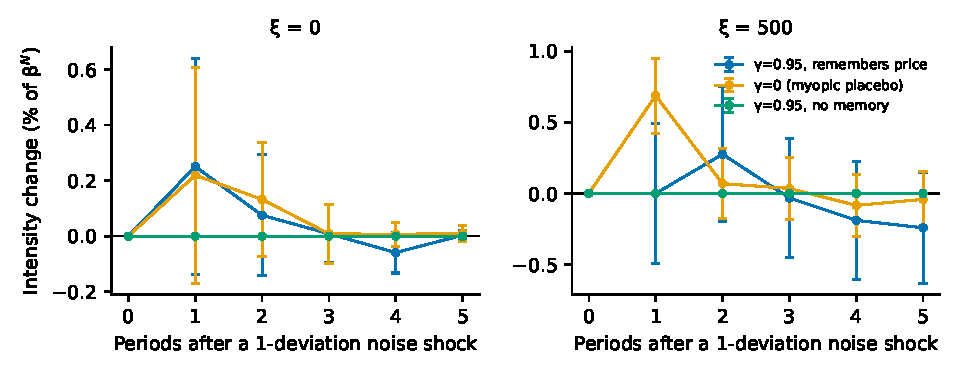
\includegraphics[width=0.9\linewidth]{figures/fig_dou.pdf}
  \caption{Noise-shock impulse responses in the \citet{dou2025} calibration
  with separate Q-tables. A noise-trader shock equal to one best-response
  deviation hits at lag 0; lines show the change in per-trader intensity in \%
  of $\beta^N$. Under price-trigger strategies intensity would jump at lag 1.}
  \label{fig:dou}
\end{figure}

\paragraph{Shared Q-tables and the placebo.} \citet{esquinas2026} find that the
price-trigger signature at $\xi=500$ is sharpest when both traders read and
update a single \emph{shared} Q-table, and that this protocol also yields
much higher collusion indices ($0.87$--$0.92$). A shared table is one learner
choosing for several traders, so we apply the same placebo to it.
Table~\ref{tab:shared} and Figure~\ref{fig:shared} show the results. Sharing
raises the index for forward-looking learners to $\SharedKyleStratDeltaInt$
($\xi=0$) and $\SharedDouStratDeltaInt$ ($\xi=500$), and for myopic learners to
$\SharedKyleMyopicDeltaInt$ and $\SharedDouMyopicDeltaInt$.

The punishment tests then fail the placebo. At $\xi=500$ the \emph{myopic}
shared learner reacts to noise shocks in proportion to their size
($\SharedDouMyopicShockSmall$, $\SharedDouMyopicShockMid$ and
$\SharedDouMyopicShockLarge\%$ of $\beta^N$ for shocks of $0.05$, $0.25$ and one
deviation unit), the threshold-and-growth pattern that \citet{dou2025} read as
a price trigger, and rivals trade harder after a forced deviation
($\SharedDouMyopicRival\pm\SharedDouMyopicRivalCI\%$ of $\beta^N$), the pattern
that \citet{calvano2020} read as punishment. A learner with $\gamma=0$ cannot
be punishing anyone, and indeed deviating still pays. The forward-looking
shared learner shows neither reaction at our horizon. The responses come from
the states the shocks and deviations lead to: they move the market into price
states that greedy play visits less often, which have been pruned less and in
which the learner therefore trades more aggressively; never-visited states keep
orders close to their Nash-like initialisation (Appendix~\ref{app:rare}).
Reactions to shocks or deviations therefore identify punishment only if a
myopic learner trained in the same way does not show them.

\paragraph{Longer training.} Because the forward-looking learner might
discover punishment only with more experience, we repeat the four
$\xi=500$ conditions with $2\times10^8$ periods per market (100 markets,
$\beta=3\times10^{-8}$, so exploration decays over the same number of
$e$-foldings), using the compiled engine. With separate tables the index
settles at $\LongSepDeltaInt$, close to the $0.31$ that \citet{esquinas2026}
report after $5\times10^8$ periods; with a shared table it rises to
$\LongSharedDeltaInt$ (theirs: $0.87$). The diagnostics do not change.
Forward-looking learners still ignore noise shocks
($\LongSharedShockLarge\pm\LongSharedShockLargeCI\%$ of $\beta^N$ after a
one-unit shock, shared; $\LongSepShockLarge\pm\LongSepShockLargeCI\%$,
separate) and forced deviations
($\LongSharedRival\pm\LongSharedRivalCI\%$ and
$\LongSepRival\pm\LongSepRivalCI\%$), and deviating pays. The myopic shared
learner, now at $\Delta=\LongSharedMyopicDeltaInt$, above its forward-looking
counterpart, still reacts to large shocks
($\LongSharedMyopicShockLarge\pm\LongSharedMyopicShockLargeCI\%$) and to
deviations ($\LongSharedMyopicRival\pm\LongSharedMyopicRivalCI\%$). Training
for thirteen times longer moves the level of the index but not what the tests
say about it.

\begin{table}[t]
  \centering
  \small
  \resizebox{\linewidth}{!}{\begin{tabular}{llcccccc}
\toprule
$\xi$ & Shared Q-table & $\Delta$ intensity & \multicolumn{3}{c}{Shock response (\% of $\beta^N$)} & Rival reaction & Seeds \\
 & & & 0.05 & 0.25 & 1 & (\% of $\beta^N$) & \\
\midrule
0 & $\gamma=0.95$ & $0.683 \pm 0.002$ & $0.10 \pm 0.11$ & $-0.02 \pm 0.24$ & $0.12 \pm 0.47$ & $0.06 \pm 0.36$ & 2 \\
0 & $\gamma=0$ (myopic placebo) & $0.856 \pm 0.001$ & $0.02 \pm 0.10$ & $0.12 \pm 0.16$ & $0.46 \pm 0.38$ & $0.06 \pm 0.31$ & 2 \\
500 & $\gamma=0.95$ & $0.618 \pm 0.002$ & $0.11 \pm 0.40$ & $0.11 \pm 0.53$ & $-0.30 \pm 0.51$ & $0.36 \pm 0.55$ & 2 \\
500 & $\gamma=0$ (myopic placebo) & $0.708 \pm 0.001$ & $0.30 \pm 0.10$ & $1.04 \pm 0.16$ & $4.01 \pm 0.22$ & $2.93 \pm 0.17$ & 2 \\
\bottomrule
\end{tabular}}
  \caption{Shared Q-tables in the \citet{dou2025} calibration
  ($1.5\times10^7$ periods, 100 markets per seed; grid-range price state at
  $\xi=500$). Shock response: change in per-trader intensity one period after
  a noise shock of the given size in deviation units. Rival reaction: change in
  rivals' intensity one period after a forced best-response deviation. Both in
  \% of $\beta^N$; 95\% CIs.}
  \label{tab:shared}
\end{table}

\begin{figure}[t]
  \centering
  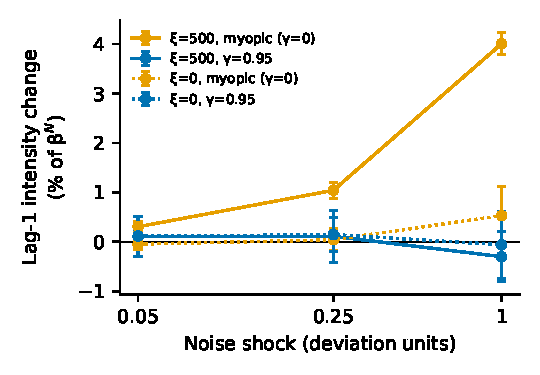
\includegraphics[width=0.5\linewidth]{figures/fig_shared.pdf}
  \caption{Noise-shock responses with shared Q-tables. At $\xi=500$ the myopic
  placebo (orange, solid) ignores small shocks and reacts increasingly to
  larger ones, the pattern read as a price trigger, although with $\gamma=0$ it
  has no reason to punish.}
  \label{fig:shared}
\end{figure}

\paragraph{The \citet{dou2025} protocol, exactly.}
\label{sec:faithful}
Our replication above follows the reimplementation of \citet{esquinas2026}.
The original differs in four respects: a step size of $\alpha=0.01$ rather
than $0.05$; exploration that decays with the number of visits to the
current value, $\varepsilon=e^{-\beta t(v)}$ with $\beta=5\times10^{-7}$,
rather than with calendar time; one common 31-point price grid rather than
bins over each value's range; and a market maker that re-estimates its rule
by least squares over a rolling window. We repeat the experiment with the
first three exactly, keeping our market maker, for $4\times10^8$ periods
(100 markets; exploration has then fallen to about $e^{-20}$), and add the
placebo and the control that \citet{dou2025} themselves use: removing the
lagged price from the state. Table~\ref{tab:faithful} reports the results;
shocks are in deviation units, $0.05$, $0.25$ and $1$ corresponding to about
2\%, 10\% and 40\% of a trader's average order (theirs: 0.25\% to 15\%).

\begin{table}[t]
  \centering
  \caption{The \citet{dou2025} protocol ($\alpha=0.01$, value-specific
  exploration with $\beta=5\times10^{-7}$, common 31-point price grid,
  $\xi=500$, $\sigma_u=0.1$ unless noted; $4\times10^8$ periods, 100 markets).
  $\Delta$ profit is their normalised profitability $\Delta_C$. Shock columns:
  change in per-trader intensity one period after a noise shock of the given
  size in deviation units; rival reaction: change in the rival's intensity one
  period after a forced best-response deviation; both in \% of $\beta^N$;
  95\% CIs.}
  \label{tab:faithful}
  \resizebox{\linewidth}{!}{\begin{tabular}{lcccccc}
\toprule
Learners ($\xi=500$) & $\Delta$ profit & $\Delta$ intensity & Shock 0.05 & Shock 0.25 & Shock 1 & Rival reaction \\
\midrule
Price memory, $\gamma=0.95$ (their baseline) & $0.29 \pm 0.01$ & $0.18 \pm 0.01$ & $0.04 \pm 0.06$ & $-0.04 \pm 0.16$ & $1.93 \pm 0.30$ & $0.23 \pm 0.19$ \\
Price memory, $\gamma=0$ (myopic placebo) & $0.12 \pm 0.01$ & $0.074 \pm 0.005$ & $0.04 \pm 0.07$ & $-0.08 \pm 0.14$ & $2.22 \pm 0.26$ & $-0.04 \pm 0.10$ \\
Lagged value only, $\gamma=0.95$ (their control) & $0.24 \pm 0.01$ & $0.143 \pm 0.005$ & $0.00 \pm 0.00$ & $0.00 \pm 0.00$ & $0.00 \pm 0.00$ & $0.00 \pm 0.00$ \\
Price memory, $\gamma=0.95$, $\sigma_u=100$ & $0.37 \pm 0.01$ & $0.24 \pm 0.01$ & $0.00 \pm 0.00$ & $0.00 \pm 0.00$ & $0.00 \pm 0.00$ & $0.00 \pm 0.00$ \\
\bottomrule
\end{tabular}}
\end{table}

Three results stand out. First, collusion is lower than in our first
replication and below the $\Delta_C\approx0.75$ that \citet{dou2025} use to
calibrate their theoretical benchmark to their simulations in this regime
(their Section 5.3): $\Delta_C=\FaDeltaProfit$ (intensity: $\FaDeltaInt$).
Their own robustness grid puts this gap in perspective (their online
appendix, Figure IA.9). At $\sigma_u=0.1$ their baseline cell
($\alpha=0.01$, $\beta=5\times10^{-7}$) gives $\Delta_C=0.7$, but three of
its four neighbours ($\beta=5\times10^{-8}$ or $5\times10^{-6}$ at the same
$\alpha$, and $\alpha=0.05$ at the same $\beta$) give $0.3$, as does most of
the grid. Our faithful run ($\FaDeltaProfit$) and our earlier runs at
$\alpha=0.05$ under the first protocol ($0.31$--$0.33$) match those
neighbouring cells. The level of
collusion in this regime is thus sensitive to the hyperparameters in their
simulations too, and our replication lands where most of their grid does. Second, the
forward-looking learner ignores shocks of 2\% and 10\% of its order, and
responds to a shock of 40\% ($\FaShockLarge\pm\FaShockLargeCI\%$ of $\beta^N$),
a threshold-like pattern; but the myopic placebo, which cannot punish,
responds in the same way and by as much
($\FaMyopicShockLarge\pm\FaMyopicShockLargeCI\%$), and a forced deviation
still pays. The rival's reaction to a deviation is small and borderline
($\FaRival\pm\FaRivalCI\%$). Third, removing the lagged price lowers
collusion only from $\FaDeltaProfit$ to $\FaNoPriceDeltaProfit$, whereas
\citet{dou2025} find that it falls to zero. With heavy noise trading
($\sigma_u=100$) collusion is higher ($\FaHighDeltaProfit$) and no reaction of
any kind appears, as they report for over-pruning, although the level is
below the $0.7$ of their corresponding cell.

\paragraph{Session by session.} An average over sessions could hide a
minority of sessions that do punish. \citet{dou2025} classify each session as
price-trigger collusion if, one period after a noise shock that moves the
price by 1.2\%, both speculators' orders rise significantly (their online
appendix, Section 4.5), and report that the pattern holds across sessions in
this regime. We apply the same rule to each of $\PsBaseSessions$ retrained
markets, averaging $\PsBaseReps$ paired replays per market, for shocks that
move the price by 0.12\%, 1.2\%, 5.5\% and 7.2\% (their small, medium, large
and ultra-large deviations). No forward-looking session qualifies at any shock
size ($\PsBaseTrigMed$\% at the medium shock, $\PsBaseTrigUltra$\% at the
largest). At the medium shock $\PsBaseFlatMed$\% of sessions show no
significant change in either trader's order, and the interquartile range of
the session responses is $[\PsBaseIqrLoMed, \PsBaseIqrHiMed]$\% of the
mean order. The only sessions the rule flags belong to the myopic placebo
($\PsMyopicTrigLarge$\% at the large shock), which cannot be punishing.

We thus do not reproduce three things: the level of collusion, its
dependence on the lagged price, and a shock response that a myopic learner
does not share.

Two differences in protocol remained. The first is their stopping rule:
each session learns until its greedy strategies are unchanged for $10^6$
consecutive periods, whereas on-path strategies in our fixed-horizon runs
still change ($\FaPolicyChange$ of entries over the last $10^7$ periods). With
their rule (capped at $2\times10^9$ periods) every session converges, after
$\SrConvMin$ to $\SrConvMax\times10^8$ periods, and nothing changes:
$\Delta_C=\SrDeltaProfit$ with the lagged price and $\SrNoPriceDeltaProfit$
without it, with the same shock and deviation responses.
The second is the market maker. We replace ours by theirs, re-estimating
$\mathbb E[v\mid y]$ by least squares over the last $10^4$ periods and pricing
$p=\hat g_0+\hat\lambda y$, so that every element of their published protocol
is matched. Again all sessions meet the stopping rule (median
$\FpConvMed\times10^8$ periods), and again nothing changes: $\Delta_C=\FpDeltaProfit$
with the lagged price and $\FpNoPriceDeltaProfit$ without it; no response to a
2\% shock ($\FpShockSmall\pm\FpShockSmallCI\%$ of $\beta^N$), a response to a
40\% shock ($\FpShockLarge\pm\FpShockLargeCI\%$) of the size the myopic placebo
also shows; no significant reaction of the rival to a forced deviation
($\FpRival\pm\FpRivalCI\%$); and deviating pays.

What we cannot reproduce is therefore the evidence that separates their
price-trigger regime from over-pruning, under an independent implementation
of every element of the protocol they describe. We do not claim that
price-trigger collusion cannot arise in their implementation; we claim that
the signatures that would identify it are not robust to an independent
implementation of the same design, and that where a trigger-like response
does appear, a learner that cannot punish shows it too.

